\chapter{ADDITIONAL TECHNICAL INFORMATION}
\label{app:add_tech_info}

\section{Mechanical Drawing}

\begin{figure}[htbp]
    \centering
    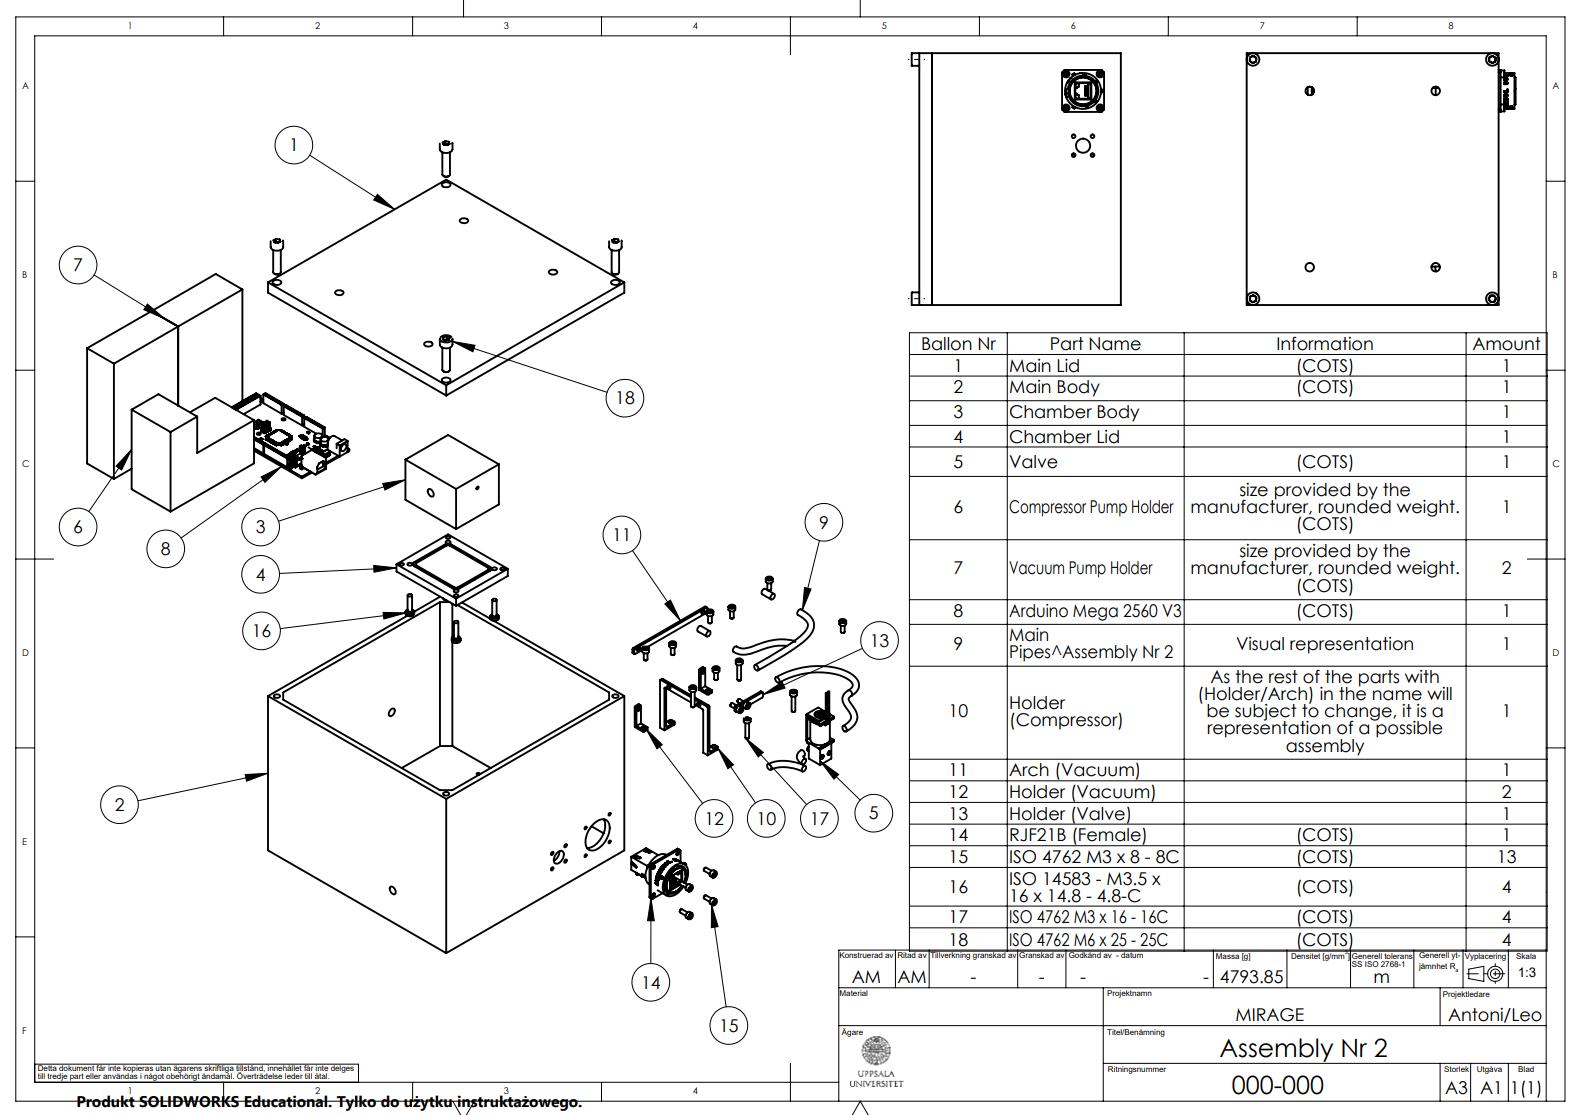
\includegraphics[angle=90, width=0.60\textheight]{0_images/figures/tech_drawing.png}
    \caption{Technical drawing of the system as a whole.}
    \label{fig:cad_system_overview}
\end{figure}

\begin{figure}[htbp]
    \centering
    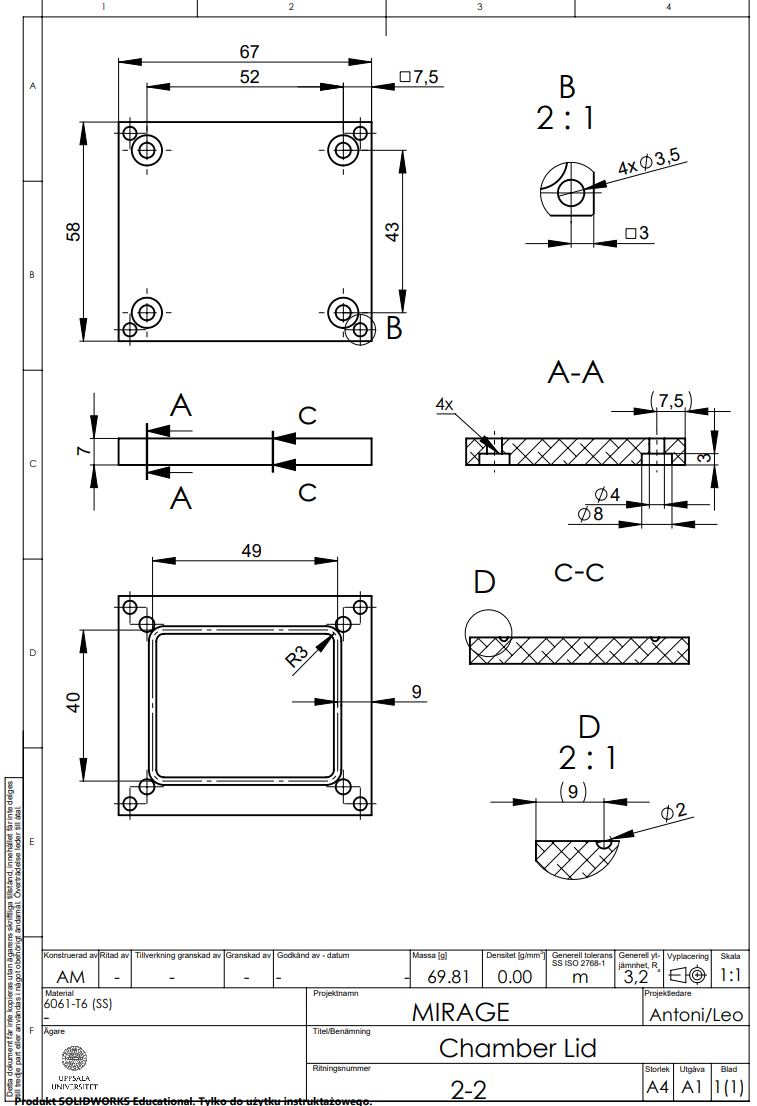
\includegraphics[angle=90, width=0.60\textheight]{0_images/figures/tech_drawing_2.png}
    \caption{Technical drawing of the pressurized chamber.}
    \label{fig:cad_pressure_chamber_1}
\end{figure}



\begin{figure}[htbp]
    \centering
    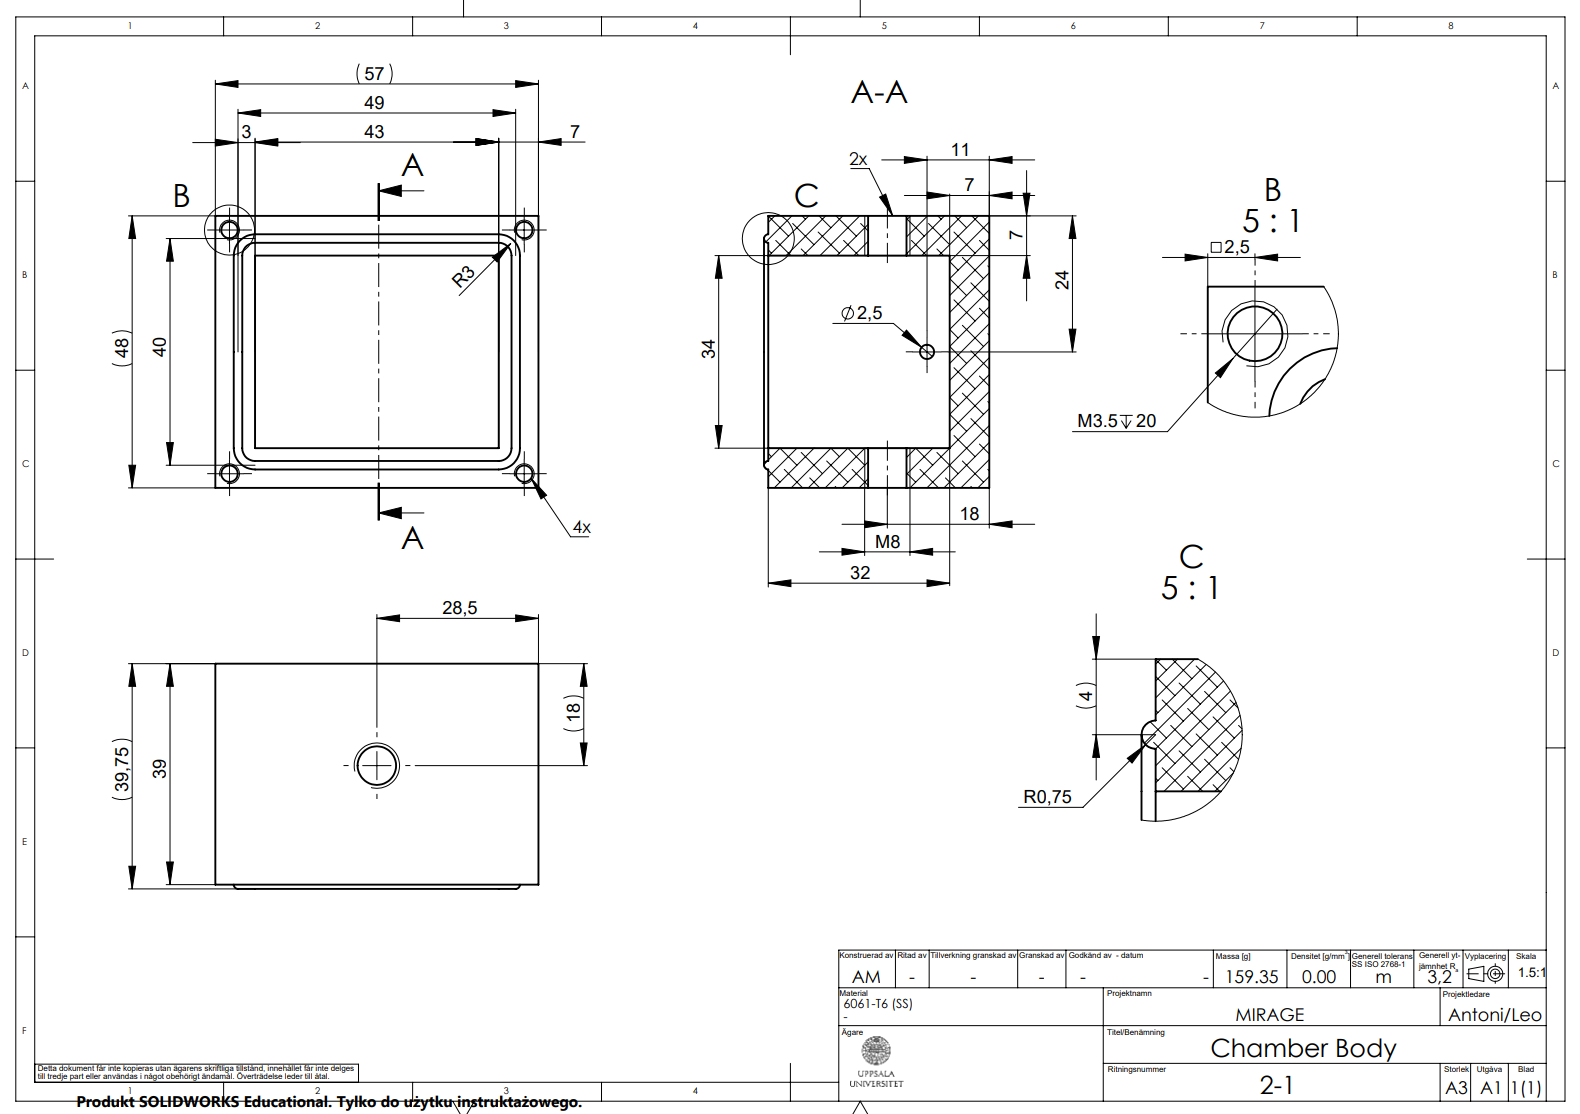
\includegraphics[angle=90, width=0.60\textheight]{0_images/figures/tech_drawing_4.png}
    \caption{Technical drawing of the pressurized chamber.}
    \label{fig:cad_pressure_chamber_2}
\end{figure}

\begin{figure}[htbp]
    \centering
    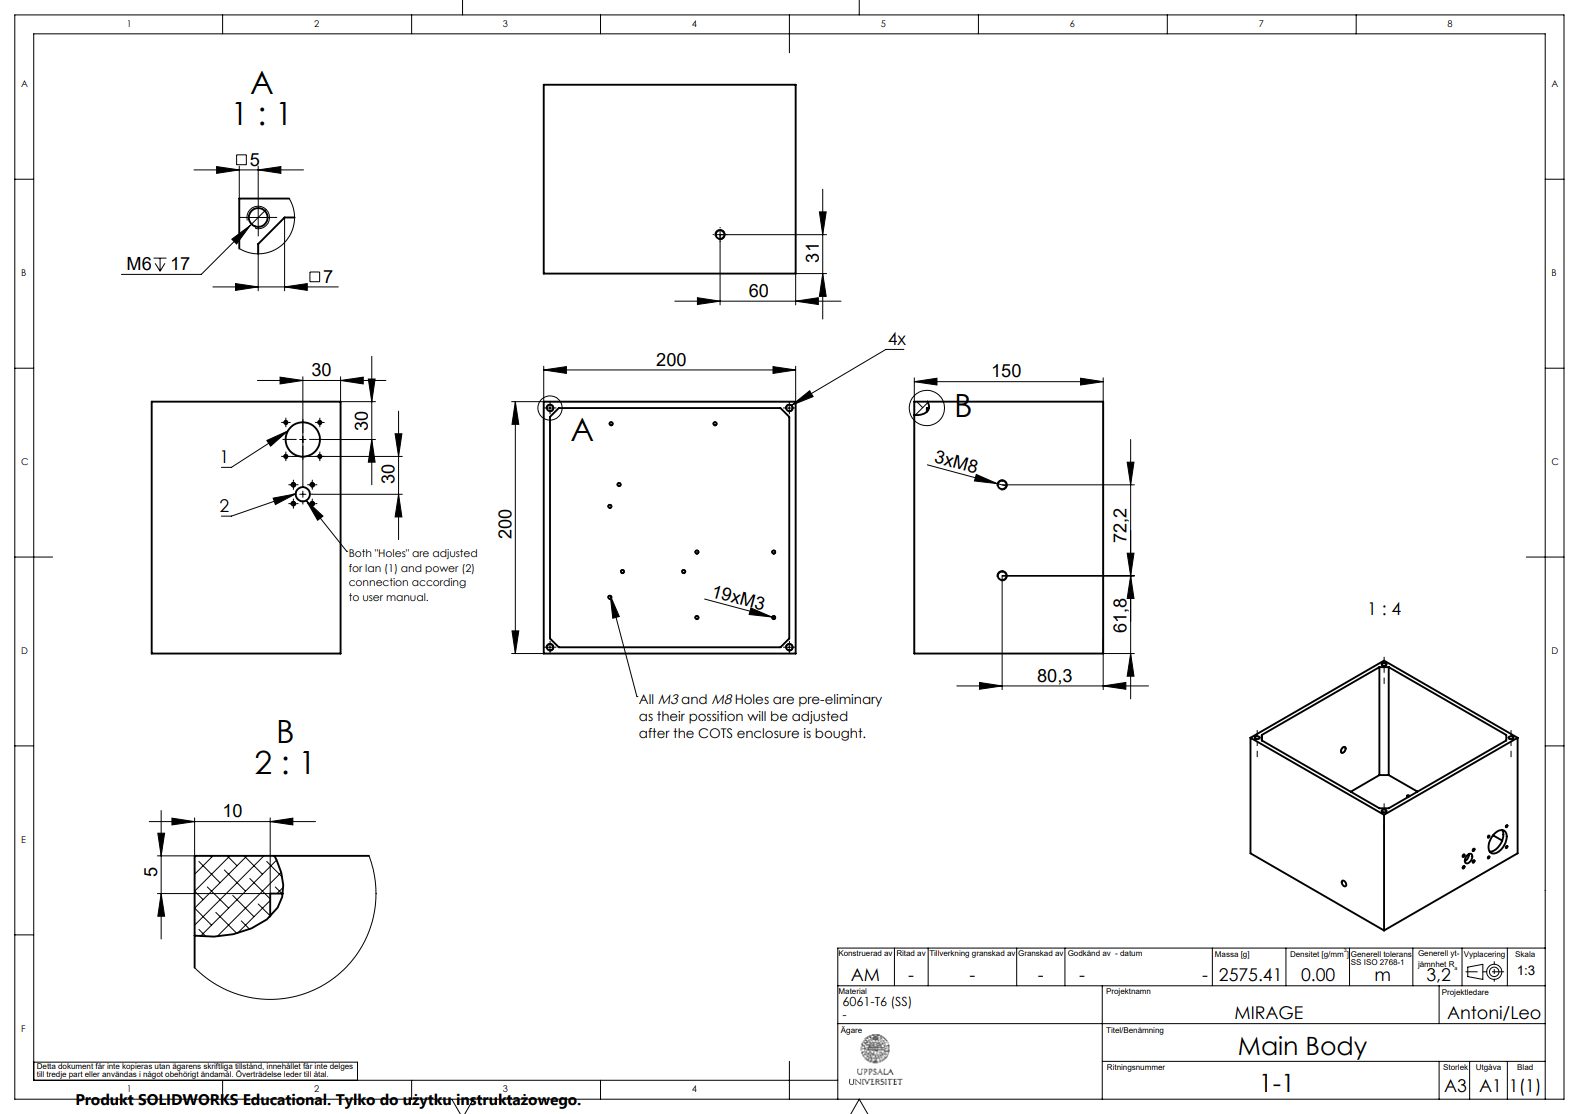
\includegraphics[angle=90, width=0.60\textheight]{0_images/figures/tech_drawing_3.png}
    \caption{Technical drawing of experiment enclosure. Drawings are representative and the thickness of both “Main Body” and “Main Lid” will be reduced to 2 mm by buying COTS parts.}
    \label{fig:cad_enclosure_1}
\end{figure}

\begin{figure}[htbp]
    \centering
    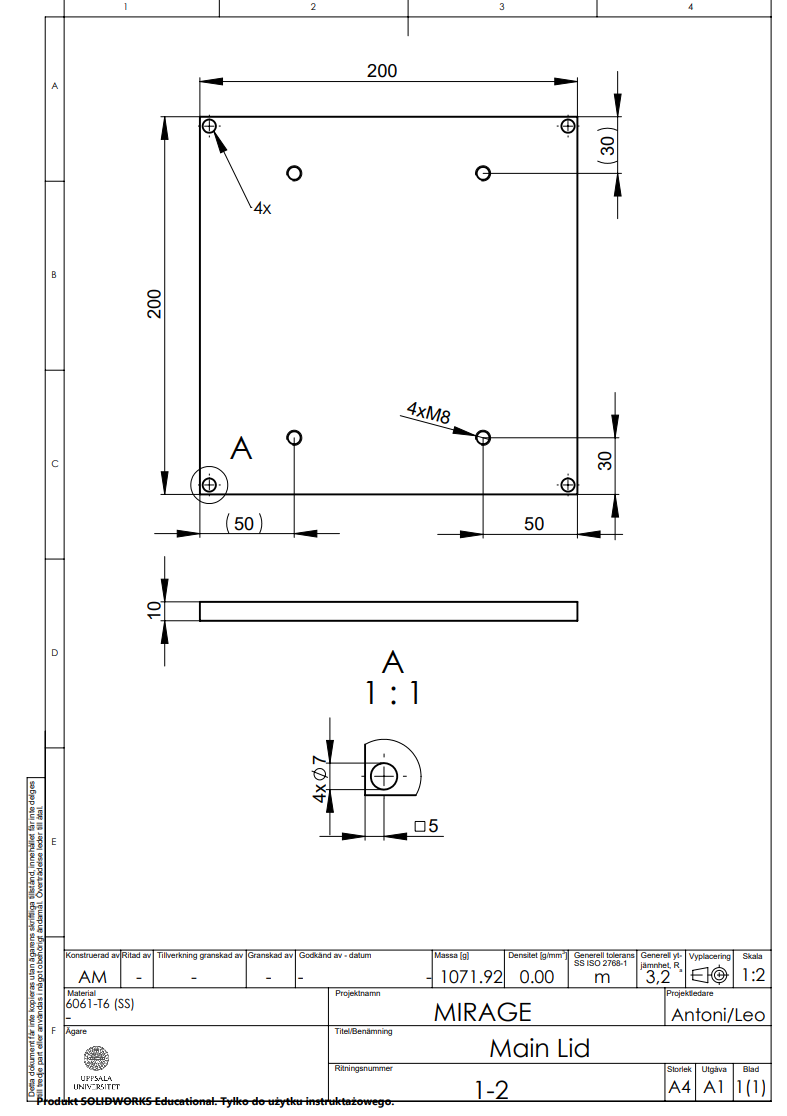
\includegraphics[angle=90, width=0.60\textheight]{0_images/figures/tech_drawing_5.png}
    \caption{Technical drawing of experiment enclosure. Drawings are representative and the thickness of both “Main Body” and “Main Lid” will be reduced to 2 mm by buying COTS parts.}
    \label{fig:cad_enclosure_2}
\end{figure}

\begin{figure}[htbp]
    \centering
    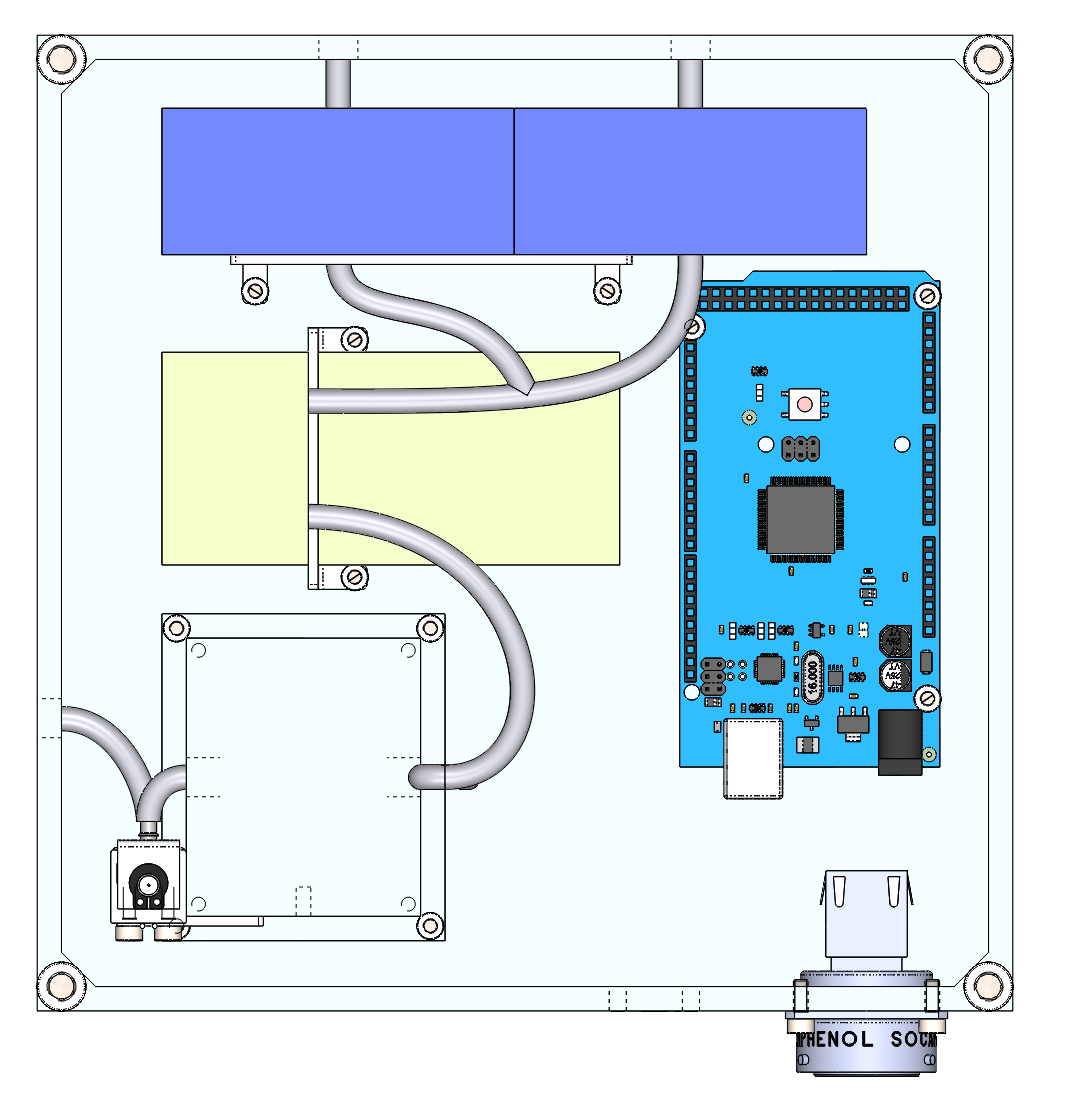
\includegraphics[angle=90, width=0.60\textheight]{0_images/figures/tech_drawing_6.png}
    \caption{Drawing of the internal layout.}
    \label{fig:cad_internal_layout}
\end{figure}

\section{Power Budget}

From secondary side and primary side:

Note that this is not taking into account duty cycles and thus 100\% duty cycle is assumed and a total operation time of 7.5h.

\begin{table}[H]
\centering
\caption{Table 1: Full flight power budget without duty cycles (100\% duty assumption)}
\label{tab:app_power_no_duty}
\resizebox{\textwidth}{!}{%
\begin{tabular}{llllllll}
\toprule
\textbf{Duration} & \textbf{Amount} & \textbf{Component} & \textbf{Voltage} & \textbf{Current} & \textbf{Power per unit} & \textbf{Total power} & \textbf{Total Energy} \\
\midrule
1.25h & 1 & K96 & 6V & 300mA & 1.8W & 2.4W & 2.25Wh \\
7.5h & 4 & SHT45 & 3.3V & 0.4$\mu$A & 1mW & 4mW & 0.03Wh \\
1.25h & 1 & Compressor & 24V & 1.25A & 30W & 30W & 37.5Wh \\
1.25h & 2 & Vacuum Pump & 24V & 0.42A & 10W & 20W & 25Wh \\
7.5h & 1 & SDHC & 3.3V & 150mA & 495mW & 495mW & 3.71Wh \\
7.5h & 1 & Main MCU & 3.3V & 175mA & 578mW & 578mW & 4.34Wh \\
7.5h & 1 & P. MCU & 3.3V & 50mA & 165mW & 165mW & 1.24Wh \\
1.33h & 1 & Peltier 2 & 3.3V & 1.52A & 5W & 5W & 6.65Wh \\
1.33h & 2 & Inlet Heater & 12V & 375mA & 4.5W & 9W & 11.97Wh \\
5h & 1 & SD-card heater & 12V & 167mA & 2W & 2W & 10Wh \\
1.33h & 1 & Chamber heater & 12V & 750mA & 9W & 9W & 11.97Wh \\
1.33h & 1 & Outlet Heater & 12V & 375mA & 4.5W & 4.5W & 5.99Wh \\
7.5h & 1 & T. MCU & 3.3V & 50mA & 165mW & 165mW & 1.24Wh \\
7.5h & 2 & MS5803 & 3.3V & 1.22mA & 4mW & 8mW & 0.06Wh \\
7.5h & 5 & TMP & 3.3V & 0.031mA & 0.1mW & 0.5mW & 4mWh \\
7.5h & 2 & ABP2 & 3.3V & 0.79mA & 2.6mW & 5.2mW & 0.04Wh \\
\midrule
Total (Average) & & & & & & 16.26W & 121.98Wh \\
Total avg (at 28.8V) & & & 28.8V & 0.66A & & 19.13W & \\
Total (at 28.8V) & & & 28.8V & & & & 143.51Wh \\
\bottomrule
\end{tabular}%
}
\end{table}

Note: Duty cycle is accounted for and the listed duty cycle is assumed during duration of use and 0\% otherwise. Some components are idle when not in use, which is accounted for. Assumptions about the pumps/compressor were: average duty cycle while active; 90\% for Vacuum Pump 1, 60\% for Vacuum Pump 2 and 70\% for compressor. These are very rough guesses and require testing.

\begin{table}[H]
\centering
\caption{Table 2: Full flight power budget with duty cycles}
\label{tab:app_power_with_duty}
\resizebox{\textwidth}{!}{%
\begin{tabular}{lllllllll}
\toprule
\textbf{Duration} & \textbf{Amount} & \textbf{Component} & \textbf{Voltage} & \textbf{Current} & \textbf{Duty Cycle} & \textbf{Power} & \textbf{Total power} & \textbf{Total Energy} \\
\midrule
1.25h & 1 & K96 & 8V & 300mA & 100\% & 2.4W & 2.4W & 2.25Wh \\
7.5h & 4 & SHT45 & 3.3V & 0.4$\mu$A & 100\% & 1mW & 4mW & 0.03Wh \\
1.25h & 1 & Compressor & 24V & 1.25A & 70\% & 30W & 30W & 26.25Wh \\
1.25h & 1 & Vacuum Pump & 24V & 0.42A & 90\% & 10W & 10W & 11.25Wh \\
1.25h & 1 & Vacuum Pump & 24V & 0.42A & 60\% & 10W & 10W & 7.5Wh \\
7.5h & 1 & SDHC & 3.3V & 150mA & 100\% & 495mW & 495mW & 3.71Wh \\
7.5h & 1 & Main MCU & 3.3V & 175mA & 100\% & 578mW & 578mW & 4.34Wh \\
1.25h & 1 & P. MCU & 3.3V & 50mA & 100\% & 165mW & 165mW & 0.21Wh \\
6.25h & 1 & P. MCU (idle) & 3.3V & 20mA & 100\% & 66mW & 66mW & 0.41Wh \\
1.33h & 1 & Peltier 2 & 3.3V & 1.52A & 20\% & 5W & 5W & 1.33Wh \\
1.33h & 1 & Inlet Heater & 12V & 375mA & 50\% & 4.5W & 9W & 5.99Wh \\
5h & 1 & SD-card heater & 12V & 167mA & 50\% & 2W & 2W & 5Wh \\
1.33h & 1 & Chamber heater & 12V & 750mA & 50\% & 9W & 9W & 5.99Wh \\
1.33h & 1 & Outlet Heater & 12V & 375mA & 10\% & 4.5W & 4.5W & 0.6Wh \\
7.5h & 1 & T. MCU & 3.3V & 50mA & 100\% & 165mW & 165mW & 1.24Wh \\
7.5h & 2 & MS5803 & 3.3V & 1.22mA & 100\% & 4mW & 8mW & 0.06Wh \\
7.5h & 5 & TMP & 3.3V & 0.031mA & 100\% & 0.1mW & 0.5mW & 4mWh \\
7.5h & 2 & ABP2 & 3.3V & 0.79mA & 100\% & 2.6mW & 5.2mW & 0.039Wh \\
1.25h & 1 & Shutter Valve & 24V & 250mA & 100\% & 6W & 6W & 7.5Wh \\
\midrule
Total (AVG) & & & & & & 11.16W & & 83.69Wh \\
Total (AVG at 28.8V) & & & & 0.46A & & 13.13W & & \\
Total (at 28.8V) & & & & & & & & 98.45Wh \\
\bottomrule
\end{tabular}%
}
\end{table}

Pre-launch (testing and ground), 3.75h duration (components are idle/standby):

\begin{table}[H]
\centering
\caption{Table 3: Pre-launch idle/standby power budget (3.75h)}
\label{tab:app_power_prelaunch_idle}
\resizebox{\textwidth}{!}{%
\begin{tabular}{lllllll}
\toprule
\textbf{Duration} & \textbf{Amount} & \textbf{Component} & \textbf{Voltage} & \textbf{Current} & \textbf{Power} & \textbf{Total Energy} \\
\midrule
3.75h & 1 & Main MCU & 3.3V & 150mA & 0.495W & 1.856Wh \\
3.75h & 1 & T.MCU & 3.3V & 20mA & 0.066W & 0.248Wh \\
3.75h & 1 & P.MCU & 3.3V & 20mA & 0.066W & 0.248Wh \\
3.75h & 1 & SDHC & 3.3V & 1mA & 3mW & 11mWh \\
\midrule
Total & & & & & & 2.36Wh \\
Total (BEXUS) & & & 28.8V & & 0.725W & 2.78Wh \\
\bottomrule
\end{tabular}%
}
\end{table}

Pre-launch T0h - T0.25h:

\begin{table}[H]
\centering
\caption{Table 4: Pre-launch T0h-T0.25h power budget}
\label{tab:app_power_prelaunch_t0}
\resizebox{\textwidth}{!}{%
\begin{tabular}{lllllllll}
\toprule
\textbf{Duration} & \textbf{Amount} & \textbf{Component} & \textbf{Voltage} & \textbf{Current} & \textbf{Duty Cycle} & \textbf{Power} & \textbf{Total power} & \textbf{Total Energy} \\
\midrule
0.25h & 5 & TMP & 3.3V & 0.031mA & 100\% & 0.1mW & 0.5mW & 0.1mWh \\
0.25h & 2 & MS5803 & 3.3V & 1.22mA & 100\% & 4mW & 8mW & 2mWh \\
0.25h & 1 & K96 & 8V & 300mA & 100\% & 2.4W & 2.4W & 0.6Wh \\
0.25h & 1 & Main MCU & 3.3V & 175mA & 100\% & 578mW & 578mW & 0.145Wh \\
0.25h & 1 & P. MCU & 3.3V & 20mA & 100\% & 66mW & 66mW & 17mWh \\
0.25h & 1 & T. MCU & 3.3V & 50mA & 100\% & 165mW & 165mW & 41mWh \\
0.25h & 3 & SHT45 & 3.3V & 0.32mA & 100\% & 1mW & 3mW & 1mWh \\
0.25h & 1 & Outlet Heater & 12V & 375mA & 10\% & 4.5W & 4.5W & 0.113Wh \\
0.25h & 1 & Inlet Heater & 12V & 375mA & 50\% & 4.5W & 4.5W & 0.563Wh \\
0.25h & 1 & SDHC & 3.3V & 150mA & 100\% & 495mW & 495mW & 0.124Wh \\
\midrule
Total (E. Side) & & & & & & & & 1.60Wh \\
Total AVG & & & & & & 6.42W & & \\
Total AVG (28.8V) & & & & & & 7.55W & & \\
Total (28.8V) & & & & & & & & 1.89Wh \\
\bottomrule
\end{tabular}%
}
\end{table}

\begin{table}[H]
\centering
\caption{Table 5: Ascent phase T0h-T1.15h}
\label{tab:app_power_ascent_peak}
\resizebox{\textwidth}{!}{%
\begin{tabular}{lllllllll}
\toprule
\textbf{Duration} & \textbf{Amount} & \textbf{Component} & \textbf{Voltage} & \textbf{Current} & \textbf{Duty Cycle} & \textbf{Power} & \textbf{Total power} & \textbf{Total Energy} \\
\midrule
1.25h & 1 & K96 & 8V & 300mA & 100\% & 2.4W & 2.4W & 3Wh \\
1.25h & 4 & SHT45 & 3.3V & 0.4$\mu$A & 100\% & 1mW & 4mW & 5mWh \\
1.25h & 1 & Compressor & 24V & 1.25A & 70\% & 30W & 30W & 26.25Wh \\
1.25h & 1 & Vacuum Pump & 24V & 0.42A & 90\% & 10W & 10W & 11.25Wh \\
1.25h & 1 & Vacuum Pump & 24V & 0.42A & 60\% & 10W & 10W & 7.50Wh \\
1.25h & 1 & SDHC & 3.3V & 150mA & 100\% & 495mW & 495mW & 0.62Wh \\
1.25h & 1 & Main MCU & 3.3V & 175mA & 100\% & 578mW & 578mW & 0.72Wh \\
1.25h & 1 & P. MCU & 3.3V & 50mA & 100\% & 165mW & 165mW & 0.21Wh \\
1.25h & 1 & Peltier 2 & 3.3V & 1.52A & 20\% & 5W & 5W & 1.25Wh \\
1.25h & 1 & Inlet Heater & 12V & 375mA & 50\% & 4.5W & 9W & 5.63Wh \\
1.25h & 1 & Chamber heater & 12V & 750mA & 50\% & 9W & 9W & 5.63Wh \\
1.25h & 1 & Outlet Heater & 12V & 375mA & 10\% & 4.5W & 4.5W & 0.56Wh \\
1.25h & 1 & T. MCU & 3.3V & 50mA & 100\% & 165mW & 165mW & 0.21Wh \\
1.25h & 2 & MS5803 & 3.3V & 1.22mA & 100\% & 4mW & 8mW & 10mWh \\
1.25h & 5 & TMP & 3.3V & 0.031mA & 100\% & 0.1mW & 0.5mW & 1mWh \\
1.25h & 2 & ABP2 & 3.3V & 0.79mA & 100\% & 2.6mW & 5.2mW & 7mWh \\
1.25h & 1 & Shutter Valve & 24V & 250mA & 100\% & 6W & 6W & 7.50Wh \\
\midrule
Total & & & & & & & & 70.34Wh \\
Total (AVG) & & & & & & 56.27W & & \\
Total & & & 28.8V & 2.30A & & & & 82.75Wh \\
Total AVG (28.8V) & & & 28.8V & & & 66.20W & & \\
\bottomrule
\end{tabular}%
}
\end{table}

\begin{table}[H]
\centering
\caption{Table 6: Ascent phase ver 2: no heaters/coolers}
\label{tab:app_power_ascent_no_thermal}
\resizebox{\textwidth}{!}{%
\begin{tabular}{lllllllll}
\toprule
\textbf{Duration} & \textbf{Amount} & \textbf{Component} & \textbf{Voltage} & \textbf{Current} & \textbf{Duty Cycle} & \textbf{Power} & \textbf{Total power} & \textbf{Total Energy} \\
\midrule
1.25h & 1 & K96 & 8V & 300mA & 100\% & 2.4W & 2.4W & 3Wh \\
1.25h & 4 & SHT45 & 3.3V & 0.4$\mu$A & 100\% & 1mW & 4mW & 5mWh \\
1.25h & 1 & Compressor & 24V & 1.25A & 70\% & 30W & 30W & 26.25Wh \\
1.25h & 1 & Vacuum Pump & 24V & 0.42A & 90\% & 10W & 10W & 11.25Wh \\
1.25h & 1 & Vacuum Pump & 24V & 0.42A & 60\% & 10W & 10W & 7.50Wh \\
1.25h & 1 & SDHC & 3.3V & 150mA & 100\% & 495mW & 495mW & 0.62Wh \\
1.25h & 1 & Main MCU & 3.3V & 175mA & 100\% & 578mW & 578mW & 0.72Wh \\
1.25h & 1 & P. MCU & 3.3V & 50mA & 100\% & 165mW & 165mW & 0.21Wh \\
1.25h & 1 & T. MCU & 3.3V & 50mA & 100\% & 165mW & 165mW & 0.21Wh \\
1.25h & 2 & MS5803 & 3.3V & 1.22mA & 100\% & 4mW & 8mW & 10mWh \\
1.25h & 5 & TMP & 3.3V & 0.031mA & 100\% & 0.1mW & 0.5mW & 1mWh \\
1.25h & 2 & ABP2 & 3.3V & 0.79mA & 100\% & 2.6mW & 5.2mW & 7mWh \\
1.25h & 1 & Shutter Valve & 24V & 250mA & 100\% & 6W & 6W & 7.50Wh \\
\midrule
Total & & & & & & & & 57.28Wh \\
Total (AVG) & & & & & & 45.82W & & \\
Total & & & 28.8V & 1.87A & & & & 67.38Wh \\
Total AVG (28.8V) & & & 28.8V & & & 53.91W & & \\
\bottomrule
\end{tabular}%
}
\end{table}